\section{Results}\label{sec:results}
\subsection{Sharpness and numerical reliability}
The population-solver validation comprises 280 cases: 14 laws at each combination of four partitions and five information-offset levels. Every state comparison agrees with the independent oracle. The largest absolute upper-risk discrepancy is $4.615\times10^{-13}$. Over the 360 partition profiles in the decision study, the largest discrepancy is $4.002\times10^{-13}$. These are numerical checks of the computed endpoints; sharpness itself follows from Theorem~\ref{thm:sharp}.

All 54 partition-coherence cases satisfy nesting, and the 18 strict-timing cases and 24 same-endpoint timing cases pass their specified checks. Recorded checks of profile decomposition, curvature, the compatibility floor and constructive completions support consistency of the implementation with the analytical identities. An independent finite-sample feasible-risk check yields 33 comparable envelopes among 40 cases, with no reported upper bound below the oracle feasible-risk diagnostic; seven cases have no oracle feasible point and provide no directional comparison. Decision-targeted and full searches agree on all 176 recorded budget comparisons. Such finite validation cannot certify all floating-point executions, but it supports the intended conservative search invariant.

\subsection{Timing changes population certification decisions}
Table~\ref{tab:population} gives a common-budget comparison for the timing-and-terminal harmful-late law. At $\rho=0.05$, every displayed partition is compatible. Endpoint information gives an upper risk of $0.065835$, exceeding $\beta=0.06$. Two bands suffice to cross the decision threshold, and further refinement lowers the upper endpoint to $0.055241$ at eight bands. The observed outcome and terminal-selection marginals are identical across these analyses.

\begin{table}[!htbp]\centering
\caption{Population decision value at $\rho=0.05$ and $\beta=0.06$ for the timing-and-terminal harmful-late law. Information quantities are in nats. A decision is a sharp population statement, without sampling uncertainty.}\label{tab:population}
\begin{tabular}{rrrrl}\toprule $K$ & $\tau_K$ & $\theta_{U,K}(0.05)$ & $\rho_K^*(0.06)$ & Decision\\\midrule
1 & 0.000000 & 0.065835 & 0.035491 & Uncertified\\
2 & 0.018323 & 0.058346 & 0.053814 & Certified\\
4 & 0.023710 & 0.055899 & 0.059201 & Certified\\
8 & 0.025106 & 0.055241 & 0.060597 & Certified\\\bottomrule\end{tabular}

\end{table}

The complete-case risk is $\td=0.037333$ and the assumption-free upper bound is $A+c=0.0975$. The eight-band compatibility floor is $0.025106$. Timing raises the certification frontier at $\beta=0.06$ from $0.035491$ at the endpoint to $0.060597$ at eight bands. The frontier difference, $0.025106$ nats, is exactly the observable timing increment. Hence, at this risk budget, the eight-band analysis changes the decision for $\rho$ in approximately $(0.035491,0.060597]$; this window lies above its compatibility floor. Figure~\ref{fig:identification} connects the profile to this sensitivity comparison.

The sensitivity budget can also be interpreted through the admissible harmful proportion among unresolved events. For the law in Table~\ref{tab:population}, the resolved harmful proportion is $A/r=0.0373$. At $\rho=0.05$, the endpoint upper-risk completion permits an unresolved harmful proportion of approximately 0.493, compared with 0.324 for eight timing bands. Relative to the resolved proportion, the corresponding harmful-outcome odds ratios are approximately 25.1 and 12.4. These quantities describe worst-case completions admitted by the assumed information budget, not estimates of the actual unresolved-outcome mechanism.

Across all 2,160 decision rows, 34 change from endpoint noncertification to refined certification: 13 for the timing-and-terminal law, 11 for high unresolvedness and 10 for timing-only selection. These are counts within a fixed design grid, not estimated probabilities of benefit. The no-path-dependence, terminal-only and low-prevalence controls produce no decision changes on this grid. At eight bands, the ordinary harmful-late law at $\rho=0.05,\beta=0.06$ remains a small-margin example: its separate confirmatory power evaluation certifies 0/100 streams by 20,000 events, as does the endpoint analysis. Its decision value is established at the population level; the next experiment addresses finite-sample value on a different, stronger-timing law.

\subsection{Finite-sample certification under informative timing}
The strong-timing law has true risk $0.02$. At $\rho=0.08$, its sharp population upper risks are $0.079617$, $0.059129$, $0.049755$ and $0.047196$ for $K=1,2,4,8$, respectively. At $\beta=0.09$, all are population-certifiable, but their margins and statistical dimensions differ substantially.

Figure~\ref{fig:power}(a) and Table~\ref{tab:power} show the resulting certification probabilities. The two-band procedure certifies 100/100 streams by 5,000 matured events, with exact 95\% interval $[0.964,1]$. Endpoint-only analysis certifies none by 5,000 and 96/100 by 50,000, with interval $[0.901,0.989]$. The 5,000-event horizon is one tenth of the 50,000-event horizon in this descriptive comparison of high observed certification frequencies. It is not a universal tenfold sample-complexity result. Four bands certify 88/100 by 5,000 and 100/100 by 10,000; eight bands certify 98/100 by 10,000. Intermediate resolution certifies earlier here, although eight bands give the smaller population bound.

The early difference is not explained solely by incomplete optimization. At 5,000 events, endpoint decision-targeted searches refuted certification in 89 of 96 streams and remained numerically unresolved in seven. The two-band procedure certified all 100 streams. At later checkpoints, unresolved numerical searches also contribute to delayed certification. The four full-search representatives are included in the headline totals but not in this targeted-search decomposition.

\begin{figure}[!htbp]
\centering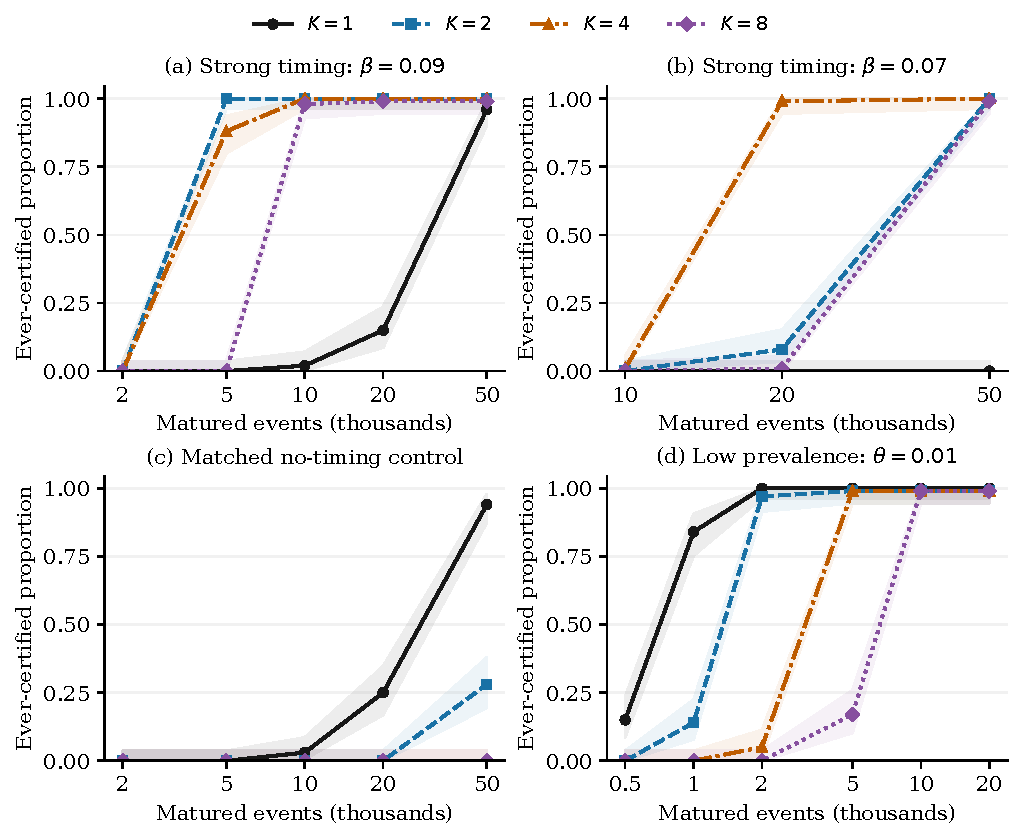
\includegraphics[width=\linewidth]{figures/certification_power.pdf}
\caption{Confirmatory certification by checkpoint, using 100 independent streams per scenario--partition cell and $\delta=0.05$ per fixed partition. Lines join observed ever-certified proportions; shaded bands are conditionwise exact two-sided 95\% Clopper--Pearson intervals. (a) Strong timing, $\rho=0.08,\beta=0.09$. (b) The same law and $\rho$, with $\beta=0.07$, below the endpoint population upper bound. (c) Matched endpoint masses with no timing contrast, $\rho=0.08,\beta=0.09$. (d) Low-prevalence law, $\rho=0.02,\beta=0.05$. Partition analyses within a law share finest-resolution streams. Checkpoints within a stream are dependent.}\label{fig:power}
\end{figure}

\begin{table}[!htbp]\centering
\caption{Selected strong-timing certification results at $\rho=0.08$. Counts refer to ever certifying by the stated horizon. Intervals quantify Monte Carlo certification probability across 100 streams, separately for each row. The full checkpoint curves and matched control are in Figure~\ref{fig:power}.}\label{tab:power}
\begin{tabular}{rrrrl}\toprule $\beta$ & $K$ & Horizon $n$ & Certified streams & Exact 95\% interval\\\midrule
0.09 & 1 & 50,000 & 96/100 & [0.9007, 0.9890]\\
0.09 & 2 & 5,000 & 100/100 & [0.9638, 1.0000]\\
0.09 & 4 & 5,000 & 88/100 & [0.7998, 0.9364]\\
0.09 & 4 & 10,000 & 100/100 & [0.9638, 1.0000]\\
0.09 & 8 & 10,000 & 98/100 & [0.9296, 0.9976]\\
0.07 & 1 & 50,000 & 0/100 & [0.0000, 0.0362]\\
0.07 & 2 & 50,000 & 100/100 & [0.9638, 1.0000]\\
0.07 & 4 & 20,000 & 99/100 & [0.9455, 0.9997]\\
0.07 & 8 & 50,000 & 99/100 & [0.9455, 0.9997]\\\bottomrule\end{tabular}

\end{table}

At the stricter $\beta=0.07$, the endpoint model is compatible but its sharp upper bound exceeds the budget. The trajectory partitions remain population-certifiable. Endpoint analysis certifies 0/100 through 50,000 events, while $K=2$ certifies 100/100 by 50,000, $K=4$ certifies 99/100 by 20,000 and 100/100 by 50,000, and $K=8$ certifies 99/100 by 50,000. Thus the comparison changes both the population decision and its finite-sample realization. Endpoint population noncertifiability is a statement about the identified set; a stochastic procedure can still issue an erroneous certificate on its confidence failure event.

The low-prevalence study provides a complementary nonvacuity check at $\theta=0.01,\rho=0.02,\beta=0.05$. Endpoint analysis certifies 100/100 by 2,000 events, two bands 97/100 by 2,000, four bands 99/100 by 5,000 and eight bands 99/100 by 10,000. Here the endpoint already has a large certification margin, so refinement does not improve the required horizons.

\subsection{When resolution pays for its statistical cost}
The matched no-timing law preserves the strong-timing law's endpoint masses but has no resolved timing information. All four population upper bounds equal $0.079617$. At 50,000 events, the certification counts are 94/100, 28/100, 0/100 and 0/100 as $K$ increases from one to eight (Figure~\ref{fig:power}c). Without informative timing, finer partitions yield lower certification frequencies in this matched control. The observed cost reflects the combined effects of categorical sampling uncertainty, aggregate-envelope relaxation and incomplete numerical search. At 50,000 events, the two-band decision-targeted searches comprise 27 current certificates, one refutation, 67 unresolved searches and one stopped path among 96 streams. The eight-band targeted searches comprise 94 refutations and two stopped paths. The four full-search representatives are accounted for separately in the reported 100-stream certification totals (Supplement). Theorem~\ref{thm:refinement} concerns population identification; it does not order finite-sample envelopes constructed with different category counts.

The additional references expose a separate trade-off. For the low-prevalence endpoint analysis at 500 events, repeated-static monitoring certifies 71/100 compared with 15/100 for TrajCert; at 1,000, the counts are 99/100 and 84/100. This power advantage comes without the time-uniform guarantee. The dense-monitoring comparison records no certification by either procedure at its risk budget; it does not demonstrate optional-stopping failure of repeated-static monitoring. In the ignorable-delay valid regime, the reference certifies 98/100 by 20,000 events; TrajCert certifies 98/100 at $K=1$ and 0/100 at $K=8$. Its stronger identification assumption explains why the reference need not pay the same sensitivity cost. Full outcomes, including noncertifying controls, are reported in the Supplement.

\subsection{Time-uniform validity diagnostics}
Table~\ref{tab:coverage} summarizes the seven retained validity scenarios. TrajCert's recorded violation diagnostic counts either an empty running region or a reported risk upper bound below the known risk. Its counts agree with the categorical-construction counts in these artifacts: one stream in the independent-resolution control, one in high unresolvedness, and none in the other five scenarios. Both nonzero diagnostics arise from empty running regions. The exact one-sided upper limits are $0.00945$ for 1/500 and $0.00597$ for 0/500, both below the configured 0.06 acceptance limit. All seven cells complete without technical failure. These conditionwise checks are consistent with the theorem but neither prove it nor establish a simultaneous 95\% campaign-level coverage statement. No scenario certifies within 500 events; certification power is evaluated separately above.

\begin{table}[!htbp]\centering
\caption{Time-uniform validity diagnostics through 500 matured events per stream, with risk projections at 100-event checkpoints. Each scenario has 500 independent streams. Limits are exact one-sided 95\% limits for the recorded ever-violation event, separately by scenario. The configured acceptance limit is 0.06, while the nominal theoretical level is $\delta=0.05$.}\label{tab:coverage}
\begin{tabular}{lrrr}\toprule Scenario & $K$ & Violations / streams & One-sided 95\% upper\\\midrule
High unresolvedness & 8 & 1/500 & 0.00945\\
Independent resolution & 8 & 1/500 & 0.00945\\
Low prevalence & 8 & 0/500 & 0.00597\\
Minimum-information completion & 8 & 0/500 & 0.00597\\
Near certification boundary & 8 & 0/500 & 0.00597\\
Near degeneracy & 8 & 0/500 & 0.00597\\
Thirty-two bands & 32 & 0/500 & 0.00597\\\bottomrule\end{tabular}

\end{table}

No false risk certification is recorded in any of the 32 power cells; zero of 100 gives a one-sided 95\% upper limit of $0.02951$ per cell. No cell with a compatible population model and a sharp upper risk above $\beta$ records a certificate. This does not imply zero error probability. Confidence-sequence exclusions of the true law range from one to six of 100 by cell, illustrating why validity is probabilistic. In the deliberately incompatible-budget cell at $K=4$, 16/100 streams certify by 20,000 even though the sensitivity assumption is false; their true risk is below $\beta$, so they are not counted as false risk certifications. No model-incompatible state was reported at the tested checkpoints, including in the two incompatible-budget cells. The finite-sample incompatibility check therefore did not detect those budget violations at the evaluated horizons. Its failure to reject cannot establish that the declared sensitivity restriction holds. These cases are retained in the Supplement and excluded from claims under a correctly specified sensitivity model.

\subsection{Computation and sensitivity boundaries}
Figure~\ref{fig:computation} separates the two computational scales. Population median runtimes are $0.419$--$0.466$ ms over $K=1$--128, with a reported median of 36 total root iterations at every $K$. Oracle discrepancies in this benchmark do not exceed $3.592\times10^{-13}$. The broader 500-event outer-projection target takes median $1.027$--$7.546$ seconds, with peak process resident memory $210.82$--$214.65$ MiB. These process-memory measurements include the Python runtime and libraries. Finite-sample projection is substantially more expensive than the scalar population solve; a conservative early return can also be less tight than the optimization target. Neither the runtime benchmark nor a node cap establishes a worst-case complexity bound for the projection.

The power-study checkpoints provide an additional operational cost measure. Across the 160 recorded checkpoint-level runtime medians, the median is 0.922 s and the maximum is 31.004 s; eleven checkpoint medians exceed 10 s. These timings exclude the four full-search representatives per cell and cover checkpoint projection-related computation rather than complete stream processing. They are distinct from the isolated scaling benchmark, and the available hardware record does not support a portable runtime comparison.

\begin{figure}[!htbp]
\centering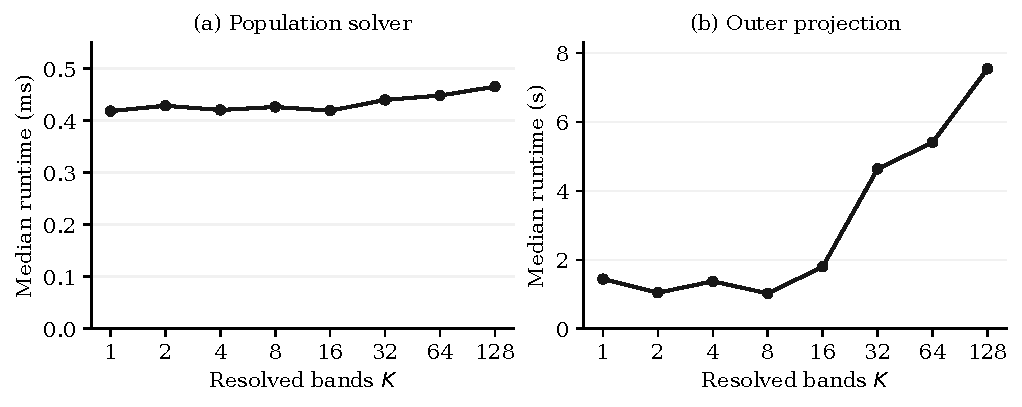
\includegraphics[width=\linewidth]{figures/computation.pdf}
\caption{Computational benchmark from existing records: medians of 30 isolated measured invocations after five warmups per $K$, with numerical-library threads limited to one. (a) Population solver, including law and summary construction. (b) Broader outer target, including a deterministic 500-event ledger, sequential confidence updates and the final projection. The law form is regenerated at each $K$, and both targets use its true information plus 0.01 nats. These curves measure cost, not nested-law information gain.}\label{fig:computation}
\end{figure}

The compatibility and risk frontiers explain the sensitivity regimes without an additional estimator. At fixed observed margins, increasing $\rho$ widens the admissible risk interval. At fixed $\rho$, refinement can either tighten a compatible interval or reveal incompatibility. An expected-count diagnostic for the low-prevalence law at $\rho=0.02,\beta=0.05$ gives upper bounds $0.0540$ at 5,000 and $0.0404$ at 10,000 events. This deterministic illustration locates a transition between those sizes; it is not a Monte Carlo estimate of certification probability.

\FloatBarrier
